\chapter{The Large Hadron Collider}

The world's largest machine is required to study the universe's smallest particles. The \ac{LHC} is circular particle collider located on the French-Swiss border outside of Geneva, Switzerland. A series of accelerators culminate in a $27$-km ring in which beams of hadrons, either protons or heavier ions, are collided. The \ac{LHC}, the most powerful hadron accelerator ever built, has been running in its current form since 2008. It is built in the tunnel previously used by \ac{LEP}, the most powerful lepton accelerator ever built, which was used to precisely measure the mass of the W and Z bosons. Collider experiments are based around the idea that $E=mc^2$: the more energetic the reaction, the more massive the particle that can be produced by it, allowing scientists to study physical phenomena not accessible in other experiments. 

There are four major experiments around the \ac{LHC} ring: \ac{ATLAS} and \ac{CMS}, general purpose detectors designed independently in order to serve as a cross-check for each other; \ac{ALICE}, a tracking-focused detector designed to study collisions of heavy ions; and \ac{LHCb}, an asymmetrical detector designed to study \ac{CP} violation. 

The dataset used in this analysis comes from proton-proton ($pp$) collisions during Run 2 of the \ac{LHC}, which spanned from 2015-2018 and had a center of mass energy of $\sqrt{s} = 13 \TeV$.

\section{Structure of the LHC}

\subsection{Acceleration}
%USED https://home.cern/science/engineering/accelerating-radiofrequency-cavities
The basic units of an accelerator are \ac{RF} cavities, used to accelerate particles, and magnets, used to focus and bend the beam. A \ac{RF} cavity is a metallic structure with an electric field that oscillates at a specified frequency. Positively charged particles are repelled from the positive field and pulled by the positive field; in the \ac{LHC}, this accelerates protons from $450 \GeV$ to $6.5 \GeV$. Once the particle reaches the required energy, it will not be further accelerated. If the proton does not have the requisite energy and arrives early or late with respect to the oscillation, it will be accelerated or decelerated by the cavity. This procedure creates a beam made of \emph{bunches} of protons, the size and spacing of which is dictated by the oscillation frequency of the accelerating cavities (at the \ac{LHC} proton bunches are $25$ ns apart)

%USED https://home.cern/science/engineering/pulling-together-superconducting-electromagnets
%USED LHC-magnets.pdf
Strong electromagnets are used to focus and bend the beam into its circular path. Superconducting \footnote{If the magnets were not superconducting, the \ac{LHC} would need to be an order of magnitude larger, $127 \textrm{km}$ in order to reach the same energy}, $14$ m long, $8.4$ T dipole magnets are required to bend the beam into its circular shape. Additional sextupole, octupole and decapole magnets accompany the dipole magnets to  correct for edge effects at their extremities. Quadrupole magnets are used to \emph{focus} the beams to squeeze them horizontally and vertically at the collision points. Careful control of the beam is extremely important for the safety of the \ac{LHC} and the detectors. 


\subsection{A Circular Proton-Proton Collider}

The history of particle physics is rich with different kinds of accelerators: linear and circular; colliding electrons, protons, and anti-protons. The \ac{LHC} is a circular, proton-proton collider -- a deliberate choice due to its physics goals. These considerations are an important part of the ongoing conversation about how the next generation of particle physics experiments should be designed. 

%USED https://home.cern/science/accelerators
First, accelerators can be linear or circular. In a linear accelerator, a particle is propelled from one end of the beam pipe to the other, increasing its energy as it goes, and eventually collides with a target or beam from another linear accelerator (or is used to feed another accelerator as in the \ac{LHC}). This means that each particle can only interact with the accelerating field once and then the particles must interact or be dumped. However, in a circular accelerator, particles make many revolutions around the acceleration path, so greater energies can be achieved in the same accelerating distance. In a circular collider, two beams of particles revolve in opposite directions and are focused at specified \ac{IP}. Particles that do not collide the first time the beams cross can be recycled and be made to collide again so collisions can happen continuously for hours. Circular electron colliders suffer from large energy loss due to synchrotron radiation due to the small mass of the electron, so the energies that can be achieved are limited (the \ac{LHC} collides protons at $\sqrt{s} = 13 \TeV$ while \ac{LEP} collided electrons and positrons at $\sqrt{s} = 209 \GeV$ in the same tunnel). In all, linear accelerators are simpler to create, but are less efficient accelerators than their circular counterparts. 

Secondly, the \ac{LHC} collides protons. Electrons are fundamental particles which create a well understood and clean collision. A collision occurs when an electron and positron annihilate. The energy produced is set by the energy of the beams and there is no ambiguity in the production mechanism of the physical process observed in the detector. Protons, however, are not fundamental particles and when two protons collide, it is their constituent quarks and gluons that interact. This means that not all of the energy of the proton is involved in the primary interaction, nor is the production mechanism known. The fraction of the proton's energy carried by the quarks and gluons is not a known quantity, it must be measured as a \ac{PDF}, which gives the probability of finding a given constituent with a given momentum. Uncertainties in \ac{PDF} measurements add to the uncertainties of the final result. This can be seen as an advantage or disadvantage: electron-positron collisions happen at a fixed energy, so they are very powerful for performing precision measurements, for example of the W and Z boson masses, where one would like many clean events where W or Z bosons were produced. In a proton-proton machine, however, a range of energy is available at each collision, making them ideal discovery environments, where one would like to look for a new particle at a wide range of masses, like in the case of the \ac{LHC} searching for the Higgs boson and \ac{BSM} phenomena. 

Additionally, the other quarks and gluons in the proton can interact as well, creating a messier collision environment compared to the electron-positron collision. Furthermore, in order to collide protons, the two beams must be separated in order for both beams to be accelerated. This is not true if one collides proton and anti-protons -- since they are oppositely charged, the same field can be used to accelerate protons in one direction and anti-protons in the other. Proton-anti-proton collisions feature more production mechanisms, but anti-protons are much harder to make and keep than protons. 







\subsection{Injection Chain}


\todo{steps of injecting}

\subsection{Using the LHC for Particle Physics}

%USED pdg-review.pdf
If the primary goal of the collider is to study rare physics processes, whether difficult measurements of the \ac{SM} or heretofore unseen \ac{BSM} physics, enough data must be produced to be able to study them. The number of events of a given process in a given data set is given by

\begin{equation}
N_{\textrm{events}} = \mathcal{L}_{\textrm{int}} \times \sigma_{\textrm{process}}
\label{eq:nevents_lumi}
\end{equation}
where $\mathcal{L}$ is the \emph{integrated luminosity} of the dataset, and $\sigma_{\textrm{process}}$ is the cross section for the given process. More data ($\mathcal{L}_{\textrm{int}}$) is required to be able to see rare events (small $\sigma_{\textrm{process}}$), and many events are required in order to have the statistical power in able to make a discovery. The integrated luminosity is the integral of the instantaneous luminosity over data taking time

\begin{equation}
\mathcal{L}_{\textrm{int}} = \int \mathcal{L} dt
\end{equation}
and the \emph{instantaneous luminosity} is related to the parameters of the accelerator. For two identical bunches with $N_1$ and $N_2$ protons per bunch colliding with frequency $f$:

\begin{equation}
\mathcal{L} = \frac{N_1 N_2 f}{4\pi \sigma_x^* \sigma_y^*} \mathcal{F}
\end{equation}
where $\sigma_x^*$ and  $\sigma_y^*$ are the \ac{rms} of the beam width in the $x$ and $y$ directions, and $\mathcal{F}$ is a factor that takes in other geometric effects such as the crossing angle and bunch length, it is generally $\mathcal{O}(1)$. It can be rewritten more specifically for the \ac{LHC} as

\begin{equation}
\mathcal{L} = \frac{N_b^2 n_b f }{4\pi \sqrt{\epsilon_n \beta^*_x \beta^*_y}}\mathcal{F}
\end{equation}
where $N_b$ is the number of protons per bunch (assuming $N_1 = N_2$), $n_b$ is the number of bunches in the beam, $\epsilon_n$ is the \emph{emittance}, which describes the spread of the particles in the bunch, and $\beta^*$ is the value of the $\beta$-function at the \ac{IP}. The $\beta$-function describes the size of the beam as a function of location. A sampling of the values of these parameters in 2018 are shown in \autoref{tab:lumi-vals}.


%USED ATLAS-lumi-measurement.pdf
% https://indico.cern.ch/event/751857/contributions/3259373/attachments/1783143/2910577/belen-Evian2019.pdf
\begin{table}
\centering
\begin{tabular}{lc}
\hline
Paramter & value  \\
\hline
$N_b$ (protons per bunch)                                           & $1.1 \times 10^{11}$   \\
$n_b$ (bunches per beam)                                            & $2544$   \\
$\beta^*$ (beam size)                                               & $.3$ m   \\
$\epsilon_n$ (beam spread)                                          & $1.8-2.2 \mu$m-radians   \\
$\mathcal{L}_{\textrm{peak}}$ (peak instantaneous luminosity)       & $21 \times 10^{33} \textrm{cm}^{-2}\textrm{s}^{-1}$   \\
space between bunches                                               & $25$ ns   \\
\hline
\end{tabular}
\caption{Beam parameters for 2018 for standard running conditions used in the data collection for this analysis. Special runs take place where these parameters are changed.}
\label{tab:lumi-vals}
\end{table}

Several of these factors can be manipulated \emph{in situ}, allowing for luminosity increasing or decreasing, depending on the need. Decreasing $\beta^*$ increases the luminosity, so the beams are \emph{squeezed} with focusing quadrupole magnets at the \ac{IP}. Nonzero beam crossing angles and longer bunches decrease luminosity. In fact, during some runs of Run 2 of the \ac{LHC}, the beam angle was changed at the beginning in order to decrease the luminosity to a level more tolerable by the experiments, referred to as \emph{leveling}. 

%The instantaneous luminosity can be measured by measuring the components directly, or it can be inferred by measuring the number of events in a process with a well measured cross section, $\sigma_{\textrm{ref}}$ that produces $N_{\textrm{ref}}$ events. By counting $N_{\textrm{exp}}$, the actual number of events produced, one can infer $\sigma_{\textrm{exp}}$. The difference between $\sigma_{\textrm{ref}}$ and $\sigma_{\textrm{exp}}$ gives information about the instantaneous luminosity from an equation similar to \autoref{eq:nevents_lumi}. 


%USED LHC-vandermeer.pdf
%USED ALTAS-lumi-measurement.pdf
In \ac{ATLAS}, luminosity is measured in two steps. First, the rate of $pp$ collisions ($\mu_{\textrm{vis}}$) is measured using detectors close to the beam pipe. This is done both online, so that adjustments to the data collection scheme can be done on the fly, as well as offline, to determine the amount of data collected. Second, the $pp$ collision rate is translated into a luminosity using a \emph{van der Meer} scan. During the scan, the beam is widened and, initially, the beams are separated in both $x$ and $y$. The beams are moved incrementally closer to each other by known amounts such that the separation between the beams is always known as the number of collisions increases. The luminosity per bunch can be expressed as

\begin{equation}
\mathcal{L}_b = \frac{\mu_{\textrm{vis}}}{\sigma_{\textrm{vis}}} f
\end{equation}
where $\mu_{\textrm{vis}}$ is measured by the luminosity detectors. The luminosity, $\mathcal{L}_b$, is known during the van der Meer scan, and so the inelastic cross section, $\sigma_{\textrm{vis}}$ can be determined and used to calculate $\mathcal{L}_b$ from $\mu_{\textrm{vis}}$. Both $\mu_{\textrm{vis}}$ and $\sigma_{\textrm{vis}}$ contain detection efficiency effects. 

%USED luminosity public results
In Run 2, the \ac{LHC} produced an integrated luminosity of $156 \textrm{fb}^{-1}$, \ac{ATLAS} recorded $147 \textrm{fb}^{-1}$, with $139 \textrm{fb}^{-1}$ available to be used for physics analyses.



\subsection{Pileup}

While high instantaneous luminosity enables the fast accumulation of data required to study rare physical processes, it also creates a dense environment in which those processes occur. The number of concurrent $pp$ collisions is called \emph{pileup}; it is substantial because the instantaneous luminosity is greater than the $pp$ inelastic scattering cross section. The average number of interactions per bunch crossing is not a static number, but the average is $33$ for all of Run 2, as seen in \autoref{fig:pileup_plot}

\begin{figure}[htbp]
\centering
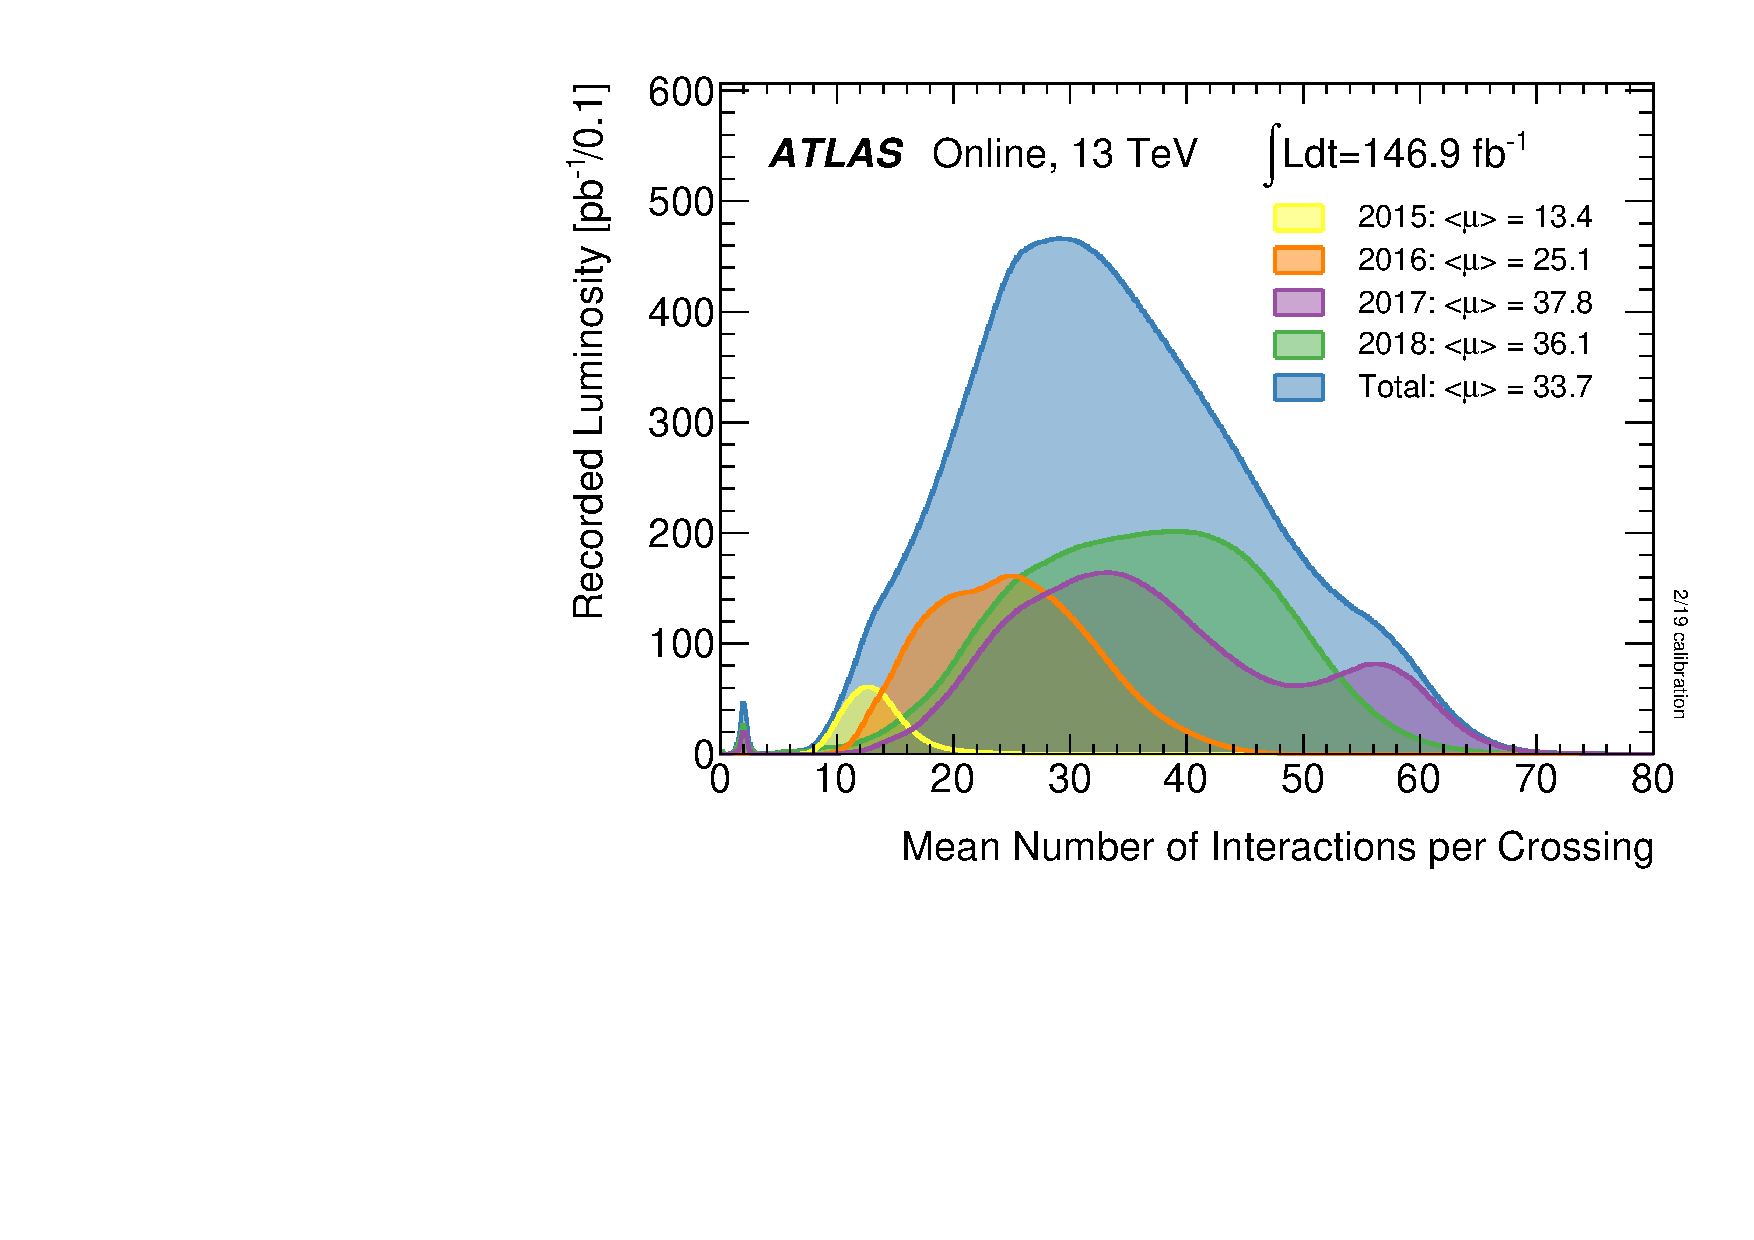
\includegraphics[width=.8\textwidth]{figures/Detector/lhc-mu.pdf}
\caption{Average number of interactions per bunch crossing during Run 2. }
\label{fig:pileup_plot}
\end{figure}

In practice, pileup collisions are generally lower energy, \ac{QCD}-only interactions, producing sprays of low energy activity in the \ac{ID} and calorimeters, which can create fake tracks, clusters, or add energy to non-pileup detector signatures.  Pileup can be mitigated by reconstructing all of the vertices in the event and removing detector signatures associated to non-primary vertices. An example of an event with 25 simultaneous collisions can be see in \autoref{fig:pileup_eventdisplay}. The tracks from the target event are the yellow lines, however there are many other tracks to confuse the situation.


\begin{figure}[htbp]
\centering
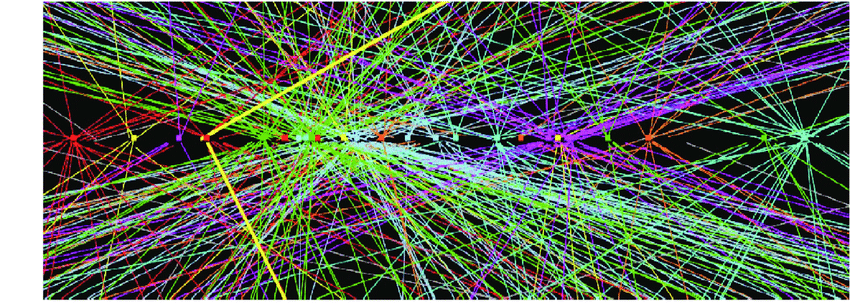
\includegraphics[width=.8\textwidth]{figures/Detector/lhc-pileup-eventdisplay.png}
\caption{An event display with 25 simultaneous interactions. The primary interaction is in yellow, but the pileup-dense environment makes it hard to see that event among all of the other activity.}
\label{fig:pileup_eventdisplay}
\end{figure}




